\documentclass[tikz,border=10pt]{standalone}
\usetikzlibrary{calc}

\begin{document}
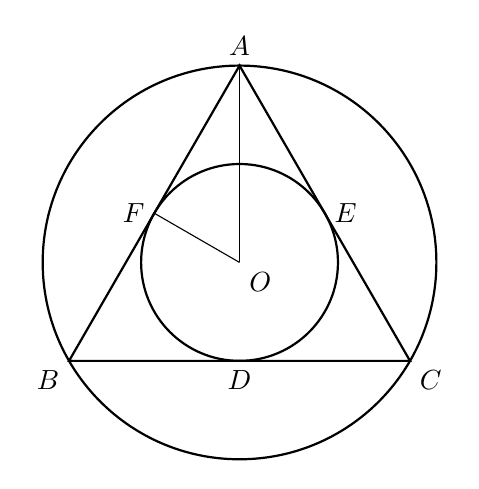
\begin{tikzpicture}
    % --- 参数定义 ---
    \def\R{2.5}  % 外接圆半径
    \def\r{1.25} % 内切圆半径 (正三角形内切圆半径为外接圆的一半)
    
    % --- 定义坐标 ---
    % 以O为原点 (0,0)
    \coordinate (O) at (0,0);
    \coordinate (A) at (90:\R);
    \coordinate (B) at (210:\R);
    \coordinate (C) at (330:\R);
    
    % 定义切点 (基于正三角形几何关系)
    \coordinate (D) at (0,-\r);   % BC的中点
    \coordinate (E) at (30:\r);   % AC上的切点
    \coordinate (F) at (150:\r);  % AB上的切点，即切点坐标方位
    
    % --- 绘制图形 ---
    % 1. 绘制外接圆
    \draw[thick] (O) circle (\R);
    
    % 2. 绘制内切圆
    \draw[thick] (O) circle (\r);
    
    % 3. 绘制三角形ABC
    \draw[thick] (A) -- (B) -- (C) -- cycle;
    
    % 4. 绘制辅助线 OA 和 OF
    \draw (O) -- (A);
    \draw (O) -- (F);
    
    % --- 标注点 ---
    \node[above] at (A) {$A$};
    \node[below left] at (B) {$B$};
    \node[below right] at (C) {$C$};
    \node[below] at (D) {$D$};
    \node[right] at (E) {$E$};
    \node[left] at (F) {$F$};
    \node[below right] at (O) {$O$};

\end{tikzpicture}
\end{document}